%%%%%%%%%%%%%%%%%%%%%%%%%%%%%%%%%%%%%%%%%
% Thin Sectioned Essay
% LaTeX Template
% Version 1.0 (3/8/13)
%
% This template has been downloaded from:
% http://www.LaTeXTemplates.com
%
% Original Author:
% Nicolas Diaz (nsdiaz@uc.cl) with extensive modifications by:
% Vel (vel@latextemplates.com)
%
% License:
% CC BY-NC-SA 3.0 (http://creativecommons.org/licenses/by-nc-sa/3.0/)
%
%%%%%%%%%%%%%%%%%%%%%%%%%%%%%%%%%%%%%%%%%

%----------------------------------------------------------------------------------------
%	PACKAGES AND OTHER DOCUMENT CONFIGURATIONS
%----------------------------------------------------------------------------------------

\documentclass[letterpaper,10pt]{article} % Font size (can be 10pt, 11pt or 12pt) and paper size (remove a4paper for US letter paper)
\usepackage{geometry}
\geometry{paperwidth=4in,margin=.1in,paperheight=27in}
\usepackage[protrusion=true,expansion=true]{microtype} % Better typography
\usepackage{graphicx} % Required for including pictures
\usepackage{caption}
\usepackage{subcaption}
\usepackage{wrapfig} % Allows in-line images
\usepackage{amsmath,amsthm}
\usepackage{thmtools}
\usepackage{xfrac}
\usepackage{mathpazo} % Use the Palatino font
\usepackage[T1]{fontenc} % Required for accented characters
\linespread{1.05} % Change line spacing here, Palatino benefits from a slight increase by default

\makeatletter
\newcommand{\pipe}{\;\middle\vert\;}
\newcommand{\condp}[2]{\Pr\left( #1 \pipe #2 \right)}
\newcommand{\pr}[1]{\Pr\left( #1 \right)}
\newcommand{\condpe}[2]{\frac{\pr{#1,#2}}{\pr{#2}}}
\newcommand{\condpb}[2]{\frac{\condp{#2}{#1}\pr{#1}}{\pr{#2}}}
\newcommand{\norm}[1]{\left|#1\right|}
\DeclareMathOperator*{\argmin}{arg\,min}
\DeclareMathOperator*{\argmax}{arg\,max}
\newcommand{\half}{\frac{1}{2}}
%theorem styling
\declaretheorem{theorem} 
\declaretheoremstyle[%
spaceabove=-6pt,%
spacebelow=6pt,%
headfont=\normalfont\itshape,%
postheadspace=1em,%
qed=\qedsymbol,%
headpunct={}
]{mystyle} 
\declaretheorem[name={},style=mystyle,unnumbered,
]{Proof}

\newcommand{\prove}[1]{
\begin{Proof}
\begin{align*}
#1
\end{align*}
\end{Proof}
}

\newcommand{\lm}{\lambda}
\newcommand{\LML}[2]{\lm #1 + (1-\lm) #2}
\newcommand{\difrac}[2]{\frac{\delta #1}{\delta #2}}
\renewcommand{\@listI}{\itemsep=0pt} % Reduce the space between items in the itemize and enumerate environments and the bibliography

\renewcommand{\maketitle}{ % Customize the title - do not edit title and author name here, see the TITLE block below
\begin{flushright} % Right align
{\LARGE\@title} % Increase the font size of the title

{\large\@author} % Author name
\\\@date % Date

\end{flushright}
}

%----------------------------------------------------------------------------------------
%	TITLE
%----------------------------------------------------------------------------------------

\title{\textbf{Assignment 3}\\ % Title
Machine Learning 10-701} % Subtitle

\author{\textsc{Arjun Menon} % Author
\\{\textit{Carnegie Mellon University}}} % Institution

%----------------------------------------------------------------------------------------

\begin{document}

\maketitle % Print the title section

\section*{Choosing an SVM Kernel}

\subsection*{2.1}

\subsubsection*{(a)}

\subsubsection*{(b)}

Decision boundaries are drawn in blue, with the red and green lines being the margins. Black squares around a data point denote a support vector. 

\begin{figure}[h]
\centering
\begin{subfigure}[b]{\textwidth}
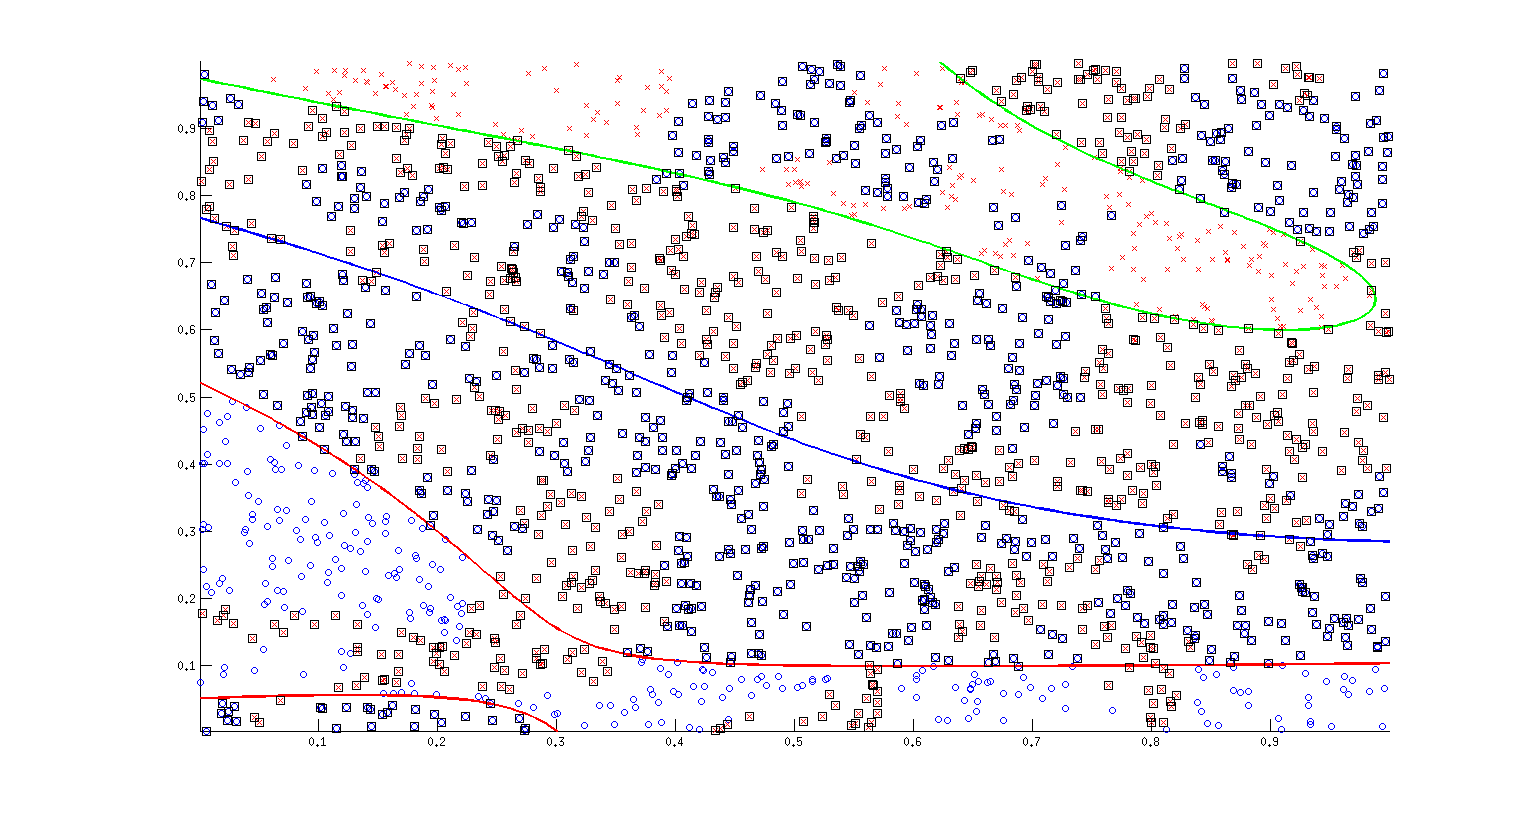
\includegraphics[width=\textwidth]{figs/p2-1a}
\caption{$\gamma = 1$}
\label{fig:p2a}
\end{subfigure}%

\begin{subfigure}[b]{\textwidth}
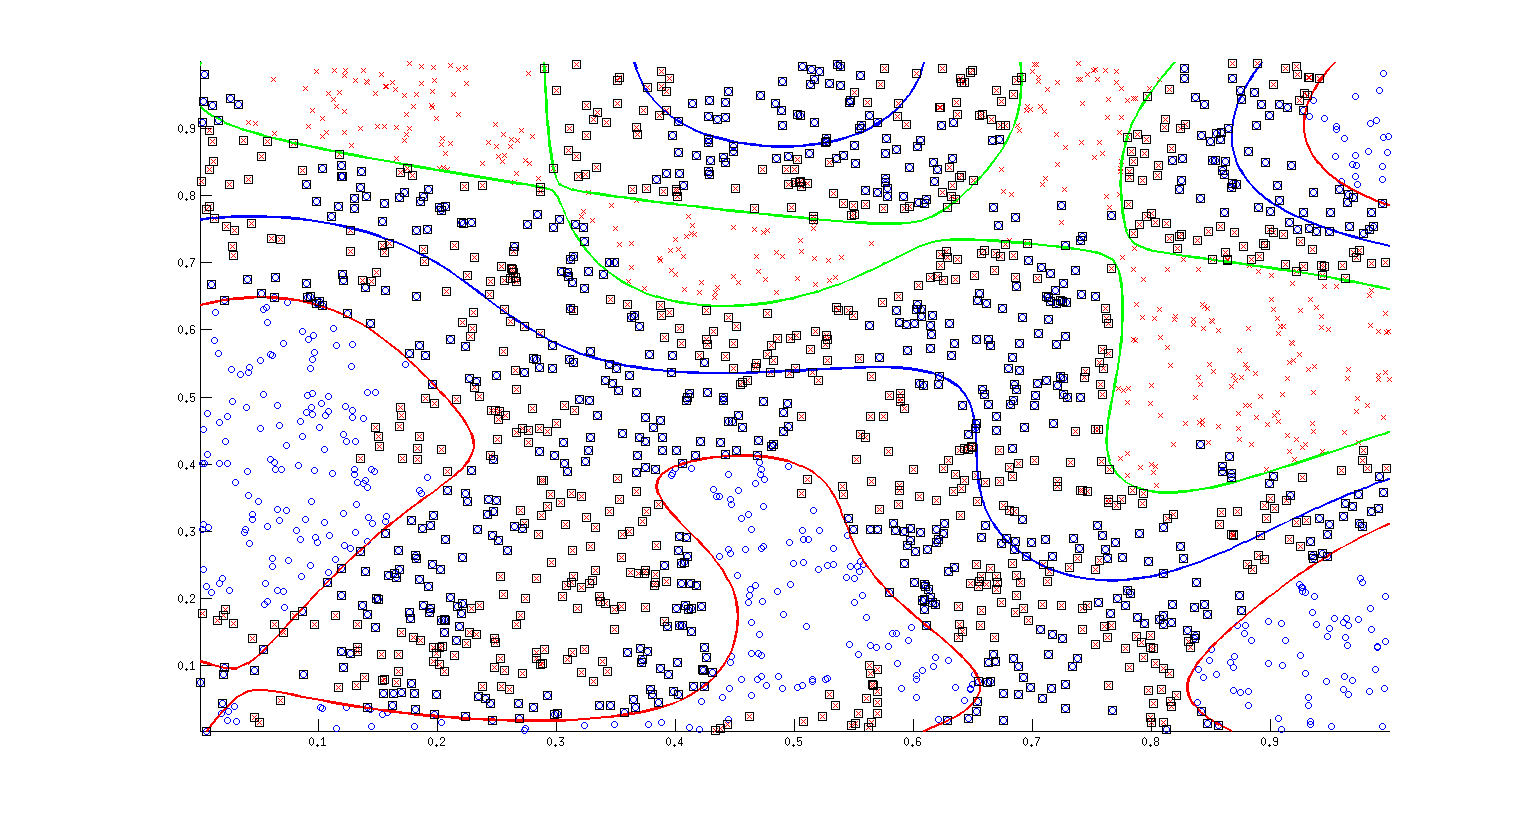
\includegraphics[width=\textwidth]{figs/p2-1b}
\caption{$\gamma = 10$}
\label{fig:p2b}
\end{subfigure}

\begin{subfigure}[b]{\textwidth}
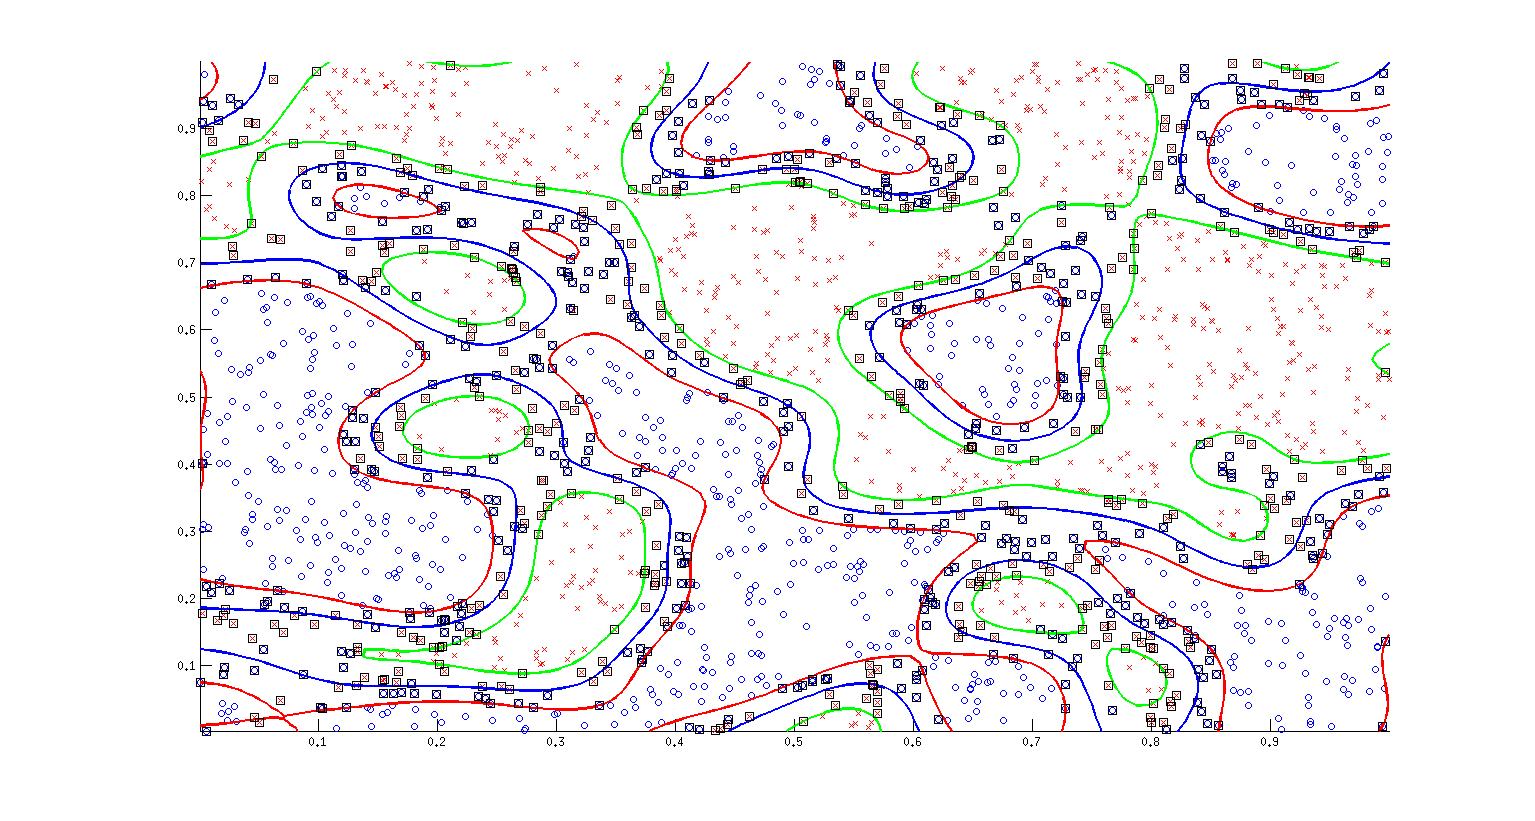
\includegraphics[width=\textwidth]{figs/p2-1c}
\caption{$\gamma = 100$}
\label{fig:p2c}
\end{subfigure}

\begin{subfigure}[b]{\textwidth}
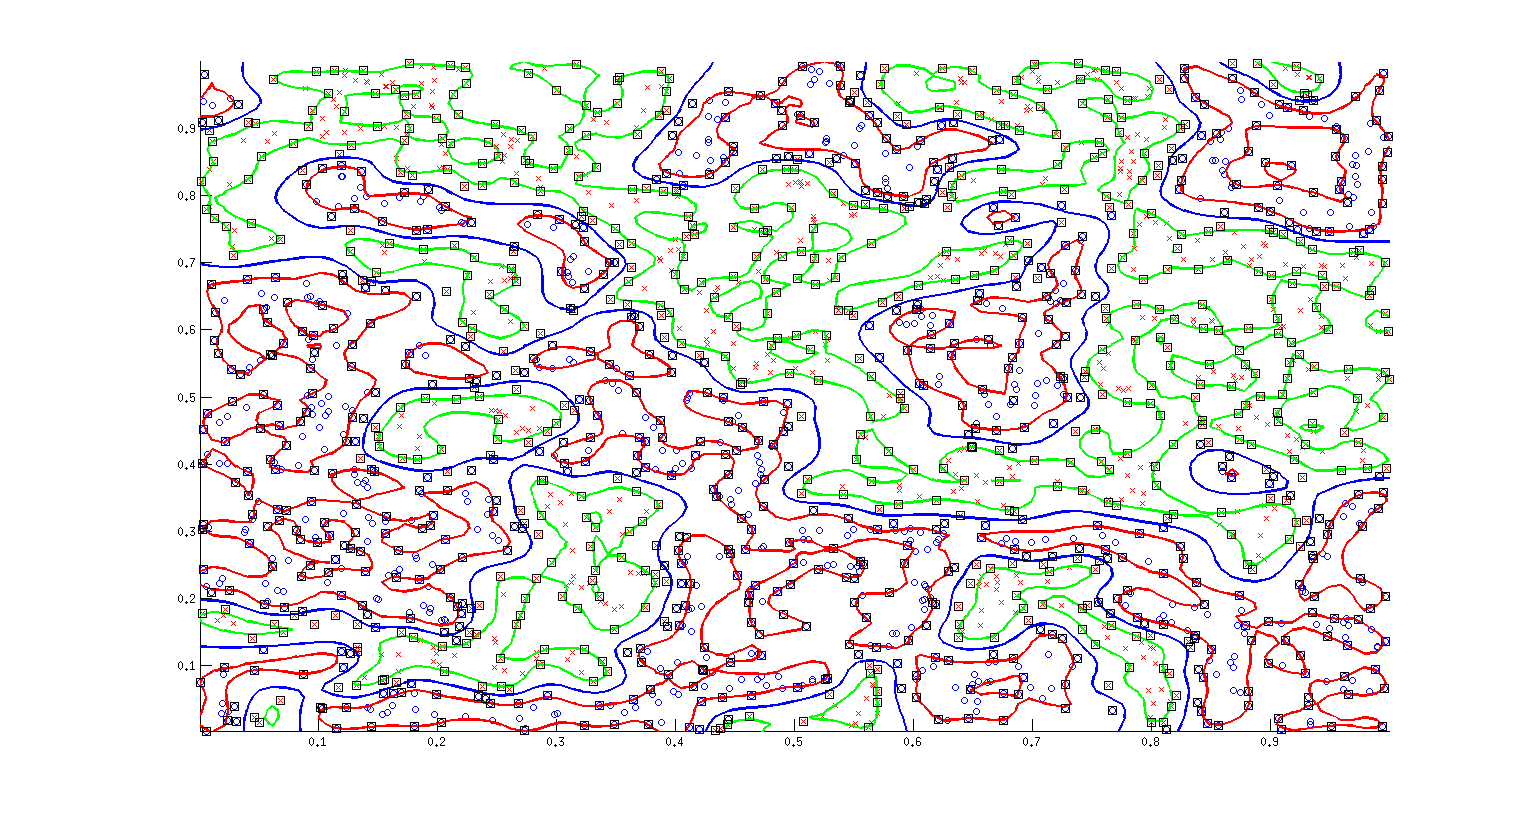
\includegraphics[width=\textwidth]{figs/p2-1d}
\caption{$\gamma = 1000$}
\label{fig:p2d}
\end{subfigure}

\begin{subfigure}[b]{\textwidth}
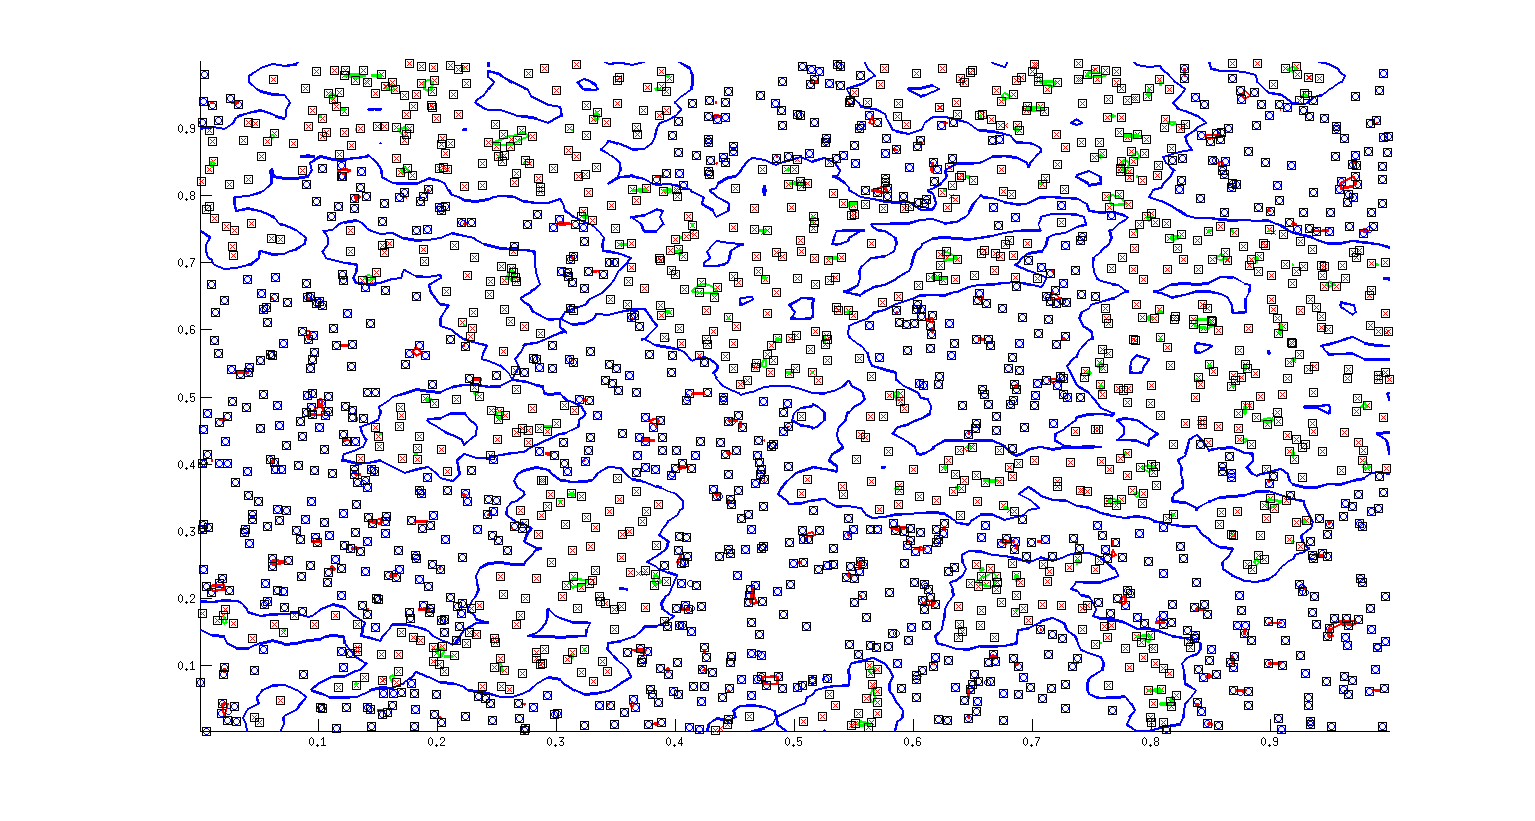
\includegraphics[width=\textwidth]{figs/p2-1e}
\caption{$\gamma = 10000$}
\label{fig:p2e}
\end{subfigure}

\caption{Differing kernel widths and their decision boundaries.}\label{fig:p2}
\end{figure}

For $\gamma = 1$, the model is underfit. For $\gamma = 10000$ the model is overfit.

For the rest in between, it remains to be seen from the testing data whether the model performs well. I personally am biased to say that $\gamma = 1000$ is also overfit, and that $\gamma = 100$ and $\gamma = 10$ would do well as the learned models since there seems to be less fragmented boundaries but still captures some of the training data.

\subsubsection*{(c)}

The best $\gamma$ is 1000, with a training error of 0.0162 and testing error of 0.0630. 

\begin{figure}[h]
\centering
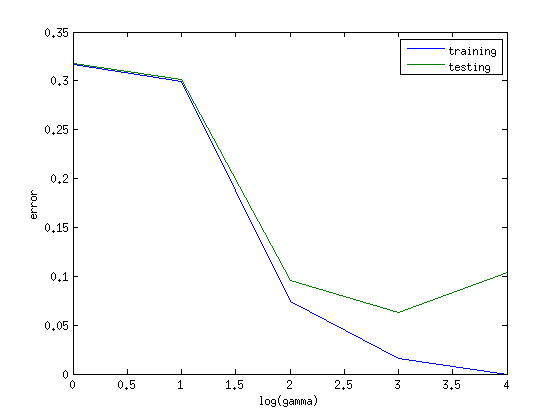
\includegraphics[width=\textwidth]{figs/p2kfold}
\caption{Comparison of training and testing error varying kernel width.}\label{fig:p2k}
\end{figure}

\subsubsection*{(d)}

It is not okay. You selected the $\gamma$ by looking at your performance on the test dataset. It doesn't fit the criteria of a blind experiment, since the information about the test itself is used to tailor your performance on it. 

\subsection*{2.2}

\subsubsection*{(a)}

Best kernel width found is 1000, with testing error of 0.0855.

\subsubsection*{(b)}

Best $K_1$ is 500 and best $K_2$ is 1000, with testing error of 0.3210.

\subsubsection*{(c)}

I would report the latter as the best estimate of the performance on holdout data. It meets the criteria for a blind experiment, where your performance won't affect your future performance. 

$K_1$ and $K_2$ do not match for me. It implies the split of the data is biased somehow towards different kernel widths. If there was more data, then the distribution fo the data in two split sets might be similar, and hence the choice of kernel width should end up matching.

%------------------------------------------------
%\bibliographystyle{unsrt}
%\bibliography{sample}

%----------------------------------------------------------------------------------------

\end{document}
